\documentclass[1p]{elsarticle_modified}
%\bibliographystyle{elsarticle-num}

%\usepackage[colorlinks]{hyperref}
%\usepackage{abbrmath_seonhwa} %\Abb, \Ascr, \Acal ,\Abf, \Afrak
\usepackage{amsfonts}
\usepackage{amssymb}
\usepackage{amsmath}
\usepackage{amsthm}
\usepackage{scalefnt}
\usepackage{amsbsy}
\usepackage{kotex}
\usepackage{caption}
\usepackage{subfig}
\usepackage{color}
\usepackage{graphicx}
\usepackage{xcolor} %% white, black, red, green, blue, cyan, magenta, yellow
\usepackage{float}
\usepackage{setspace}
\usepackage{hyperref}

\usepackage{tikz}
\usetikzlibrary{arrows}

\usepackage{multirow}
\usepackage{array} % fixed length table
\usepackage{hhline}

%%%%%%%%%%%%%%%%%%%%%
\makeatletter
\renewcommand*\env@matrix[1][\arraystretch]{%
	\edef\arraystretch{#1}%
	\hskip -\arraycolsep
	\let\@ifnextchar\new@ifnextchar
	\array{*\c@MaxMatrixCols c}}
\makeatother %https://tex.stackexchange.com/questions/14071/how-can-i-increase-the-line-spacing-in-a-matrix
%%%%%%%%%%%%%%%

\usepackage[normalem]{ulem}

\newcommand{\msout}[1]{\ifmmode\text{\sout{\ensuremath{#1}}}\else\sout{#1}\fi}
%SOURCE: \msout is \stkout macro in https://tex.stackexchange.com/questions/20609/strikeout-in-math-mode

\newcommand{\cancel}[1]{
	\ifmmode
	{\color{red}\msout{#1}}
	\else
	{\color{red}\sout{#1}}
	\fi
}

\newcommand{\add}[1]{
	{\color{blue}\uwave{#1}}
}

\newcommand{\replace}[2]{
	\ifmmode
	{\color{red}\msout{#1}}{\color{blue}\uwave{#2}}
	\else
	{\color{red}\sout{#1}}{\color{blue}\uwave{#2}}
	\fi
}

\newcommand{\Sol}{\mathcal{S}} %segment
\newcommand{\D}{D} %diagram
\newcommand{\A}{\mathcal{A}} %arc


%%%%%%%%%%%%%%%%%%%%%%%%%%%%%5 test

\def\sl{\operatorname{\textup{SL}}(2,\Cbb)}
\def\psl{\operatorname{\textup{PSL}}(2,\Cbb)}
\def\quan{\mkern 1mu \triangleright \mkern 1mu}

\theoremstyle{definition}
\newtheorem{thm}{Theorem}[section]
\newtheorem{prop}[thm]{Proposition}
\newtheorem{lem}[thm]{Lemma}
\newtheorem{ques}[thm]{Question}
\newtheorem{cor}[thm]{Corollary}
\newtheorem{defn}[thm]{Definition}
\newtheorem{exam}[thm]{Example}
\newtheorem{rmk}[thm]{Remark}
\newtheorem{alg}[thm]{Algorithm}

\newcommand{\I}{\sqrt{-1}}
\begin{document}

%\begin{frontmatter}
%
%\title{Boundary parabolic representations of knots up to 8 crossings}
%
%%% Group authors per affiliation:
%\author{Yunhi Cho} 
%\address{Department of Mathematics, University of Seoul, Seoul, Korea}
%\ead{yhcho@uos.ac.kr}
%
%
%\author{Seonhwa Kim} %\fnref{s_kim}}
%\address{Center for Geometry and Physics, Institute for Basic Science, Pohang, 37673, Korea}
%\ead{ryeona17@ibs.re.kr}
%
%\author{Hyuk Kim}
%\address{Department of Mathematical Sciences, Seoul National University, Seoul 08826, Korea}
%\ead{hyukkim@snu.ac.kr}
%
%\author{Seokbeom Yoon}
%\address{Department of Mathematical Sciences, Seoul National University, Seoul, 08826,  Korea}
%\ead{sbyoon15@snu.ac.kr}
%
%\begin{abstract}
%We find all boundary parabolic representation of knots up to 8 crossings.
%
%\end{abstract}
%\begin{keyword}
%    \MSC[2010] 57M25 
%\end{keyword}
%
%\end{frontmatter}

%\linenumbers
%\tableofcontents
%
\newcommand\colored[1]{\textcolor{white}{\rule[-0.35ex]{0.8em}{1.4ex}}\kern-0.8em\color{red} #1}%
%\newcommand\colored[1]{\textcolor{white}{ #1}\kern-2.17ex	\textcolor{white}{ #1}\kern-1.81ex	\textcolor{white}{ #1}\kern-2.15ex\color{red}#1	}

{\Large $\underline{11n_{126}~(K11n_{126})}$}

\setlength{\tabcolsep}{10pt}
\renewcommand{\arraystretch}{1.6}
\vspace{1cm}\begin{tabular}{m{100pt}>{\centering\arraybackslash}m{274pt}}
\multirow{5}{120pt}{
	\centering
	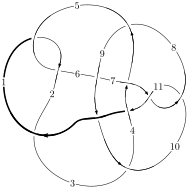
\includegraphics[width=112pt]{../../../GIT/diagram.site/Diagrams/png/742_11n_126.png}\\
\ \ \ A knot diagram\footnotemark}&
\allowdisplaybreaks
\textbf{Linearized knot diagam} \\
\cline{2-2}
 &
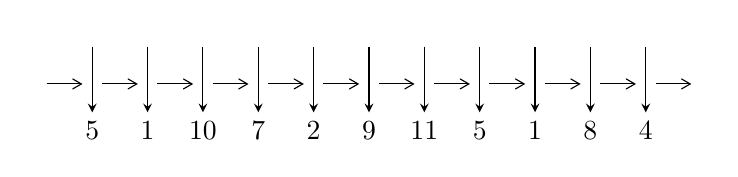
\begin{tikzpicture}[x=20pt, y=17pt]
	% nodes
	\node (C0) at (0, 0) {};
	\node (C1) at (1, 0) {};
	\node (C1U) at (1, +1) {};
	\node (C1D) at (1, -1) {5};

	\node (C2) at (2, 0) {};
	\node (C2U) at (2, +1) {};
	\node (C2D) at (2, -1) {1};

	\node (C3) at (3, 0) {};
	\node (C3U) at (3, +1) {};
	\node (C3D) at (3, -1) {10};

	\node (C4) at (4, 0) {};
	\node (C4U) at (4, +1) {};
	\node (C4D) at (4, -1) {7};

	\node (C5) at (5, 0) {};
	\node (C5U) at (5, +1) {};
	\node (C5D) at (5, -1) {2};

	\node (C6) at (6, 0) {};
	\node (C6U) at (6, +1) {};
	\node (C6D) at (6, -1) {9};

	\node (C7) at (7, 0) {};
	\node (C7U) at (7, +1) {};
	\node (C7D) at (7, -1) {11};

	\node (C8) at (8, 0) {};
	\node (C8U) at (8, +1) {};
	\node (C8D) at (8, -1) {5};

	\node (C9) at (9, 0) {};
	\node (C9U) at (9, +1) {};
	\node (C9D) at (9, -1) {1};

	\node (C10) at (10, 0) {};
	\node (C10U) at (10, +1) {};
	\node (C10D) at (10, -1) {8};

	\node (C11) at (11, 0) {};
	\node (C11U) at (11, +1) {};
	\node (C11D) at (11, -1) {4};
	\node (C12) at (12, 0) {};

	% arrows
	\draw[->,>={angle 60}]
	(C0) edge (C1) (C1) edge (C2) (C2) edge (C3) (C3) edge (C4) (C4) edge (C5) (C5) edge (C6) (C6) edge (C7) (C7) edge (C8) (C8) edge (C9) (C9) edge (C10) (C10) edge (C11) (C11) edge (C12) ;	\draw[->,>=stealth]
	(C1U) edge (C1D) (C2U) edge (C2D) (C3U) edge (C3D) (C4U) edge (C4D) (C5U) edge (C5D) (C6U) edge (C6D) (C7U) edge (C7D) (C8U) edge (C8D) (C9U) edge (C9D) (C10U) edge (C10D) (C11U) edge (C11D) ;
	\end{tikzpicture} \\
\hhline{~~} \\& 
\textbf{Solving Sequence} \\ \cline{2-2} 
 &
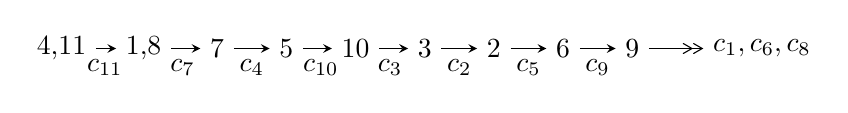
\begin{tikzpicture}[x=25pt, y=7pt]
	% node
	\node (A0) at (-1/8, 0) {4,11};
	\node (A1) at (17/16, 0) {1,8};
	\node (A2) at (17/8, 0) {7};
	\node (A3) at (25/8, 0) {5};
	\node (A4) at (33/8, 0) {10};
	\node (A5) at (41/8, 0) {3};
	\node (A6) at (49/8, 0) {2};
	\node (A7) at (57/8, 0) {6};
	\node (A8) at (65/8, 0) {9};
	\node (C1) at (1/2, -1) {$c_{11}$};
	\node (C2) at (13/8, -1) {$c_{7}$};
	\node (C3) at (21/8, -1) {$c_{4}$};
	\node (C4) at (29/8, -1) {$c_{10}$};
	\node (C5) at (37/8, -1) {$c_{3}$};
	\node (C6) at (45/8, -1) {$c_{2}$};
	\node (C7) at (53/8, -1) {$c_{5}$};
	\node (C8) at (61/8, -1) {$c_{9}$};
	\node (A9) at (10, 0) {$c_{1},c_{6},c_{8}$};

	% edge
	\draw[->,>=stealth]	
	(A0) edge (A1) (A1) edge (A2) (A2) edge (A3) (A3) edge (A4) (A4) edge (A5) (A5) edge (A6) (A6) edge (A7) (A7) edge (A8) ;
	\draw[->>,>={angle 60}]	
	(A8) edge (A9);
\end{tikzpicture} \\ 

\end{tabular} \\

\footnotetext{
The image of knot diagram is generated by the software ``\textbf{Draw programme}" developed by Andrew Bartholomew(\url{http://www.layer8.co.uk/maths/draw/index.htm\#Running-draw}), where we modified some parts for our purpose(\url{https://github.com/CATsTAILs/LinksPainter}).
}\phantom \\ \newline 
\centering \textbf{Ideals for irreducible components\footnotemark of $X_{\text{par}}$} 
 
\begin{align*}
I^u_{1}&=\langle 
b+u,\;a- u-1,\;u^5+2 u^4+4 u^3+2 u^2+2 u-1\rangle \\
I^u_{2}&=\langle 
b+u,\;a- u+1,\;u^4- u^3+u^2+u-1\rangle \\
I^u_{3}&=\langle 
b+u,\;u^5+u^3+u^2+a,\;u^6- u^5+2 u^4- u^3+2 u^2-2 u+1\rangle \\
I^u_{4}&=\langle 
- u^5-3 u^4-4 u^3-3 u^2+b-3 u-1,\;u^5+4 u^4+7 u^3+7 u^2+2 a+6 u+4,\\
\phantom{I^u_{4}}&\phantom{= \langle  }u^6+4 u^5+7 u^4+7 u^3+6 u^2+4 u+2\rangle \\
I^u_{5}&=\langle 
- u^5+u^4-2 u^3+u^2+b-2 u+1,\;u^5- u^4+2 u^3- u^2+a+2 u-2,\;u^6- u^5+2 u^4- u^3+2 u^2-2 u+1\rangle \\
I^u_{6}&=\langle 
b- u+1,\;a+u,\;u^2+1\rangle \\
I^u_{7}&=\langle 
b- u+1,\;2 a+u-2,\;u^2-2 u+2\rangle \\
I^u_{8}&=\langle 
b+u,\;a-2 u-1,\;u^2+1\rangle \\
\\
\end{align*}
\raggedright * 8 irreducible components of $\dim_{\mathbb{C}}=0$, with total 33 representations.\\
\footnotetext{All coefficients of polynomials are rational numbers. But the coefficients are sometimes approximated in decimal forms when there is not enough margin.}
\newpage
\renewcommand{\arraystretch}{1}
\centering \section*{I. $I^u_{1}= \langle b+u,\;a- u-1,\;u^5+2 u^4+4 u^3+2 u^2+2 u-1 \rangle$}
\flushleft \textbf{(i) Arc colorings}\\
\begin{tabular}{m{7pt} m{180pt} m{7pt} m{180pt} }
\flushright $a_{4}=$&$\begin{pmatrix}0\\u\end{pmatrix}$ \\
\flushright $a_{11}=$&$\begin{pmatrix}1\\0\end{pmatrix}$ \\
\flushright $a_{1}=$&$\begin{pmatrix}1\\u^2\end{pmatrix}$ \\
\flushright $a_{8}=$&$\begin{pmatrix}u+1\\- u\end{pmatrix}$ \\
\flushright $a_{7}=$&$\begin{pmatrix}1\\- u\end{pmatrix}$ \\
\flushright $a_{5}=$&$\begin{pmatrix}- u\\u^2+u\end{pmatrix}$ \\
\flushright $a_{10}=$&$\begin{pmatrix}u^2+u+1\\- u^2\end{pmatrix}$ \\
\flushright $a_{3}=$&$\begin{pmatrix}- u^3- u+1\\u^4+3 u^3+2 u^2+3 u-1\end{pmatrix}$ \\
\flushright $a_{2}=$&$\begin{pmatrix}- u^4- u^3- u^2+1\\-2 u^3-2 u+1\end{pmatrix}$ \\
\flushright $a_{6}=$&$\begin{pmatrix}2 u^4+2 u^3+2 u^2-1\\5 u^3+2 u^2+6 u-2\end{pmatrix}$ \\
\flushright $a_{9}=$&$\begin{pmatrix}- u^4- u^3- u^2+u+1\\-2 u^3- u^2-3 u+1\end{pmatrix}$\\ \flushright $a_{9}=$&$\begin{pmatrix}- u^4- u^3- u^2+u+1\\-2 u^3- u^2-3 u+1\end{pmatrix}$\\&\end{tabular}
\flushleft \textbf{(ii) Obstruction class $= -1$}\\~\\
\flushleft \textbf{(iii) Cusp Shapes $= -3 u^4-9 u^3-12 u^2-9 u-9$}\\~\\
\newpage\renewcommand{\arraystretch}{1}
\flushleft \textbf{(iv) u-Polynomials at the component}\newline \\
\begin{tabular}{m{50pt}|m{274pt}}
Crossings & \hspace{64pt}u-Polynomials at each crossing \\
\hline $$\begin{aligned}c_{1},c_{3},c_{5}\\c_{8}\end{aligned}$$&$\begin{aligned}
&u^5+4 u^4+3 u^3-2 u^2+u+1
\end{aligned}$\\
\hline $$\begin{aligned}c_{2}\end{aligned}$$&$\begin{aligned}
&u^5+10 u^4+27 u^3+6 u^2+5 u+1
\end{aligned}$\\
\hline $$\begin{aligned}c_{4},c_{7},c_{10}\\c_{11}\end{aligned}$$&$\begin{aligned}
&u^5-2 u^4+4 u^3-2 u^2+2 u+1
\end{aligned}$\\
\hline $$\begin{aligned}c_{6},c_{9}\end{aligned}$$&$\begin{aligned}
&u^5-6 u^4+12 u^3-9 u^2+5 u+2
\end{aligned}$\\
\hline
\end{tabular}\\~\\
\newpage\renewcommand{\arraystretch}{1}
\flushleft \textbf{(v) Riley Polynomials at the component}\newline \\
\begin{tabular}{m{50pt}|m{274pt}}
Crossings & \hspace{64pt}Riley Polynomials at each crossing \\
\hline $$\begin{aligned}c_{1},c_{3},c_{5}\\c_{8}\end{aligned}$$&$\begin{aligned}
&y^5-10 y^4+27 y^3-6 y^2+5 y-1
\end{aligned}$\\
\hline $$\begin{aligned}c_{2}\end{aligned}$$&$\begin{aligned}
&y^5-46 y^4+619 y^3+214 y^2+13 y-1
\end{aligned}$\\
\hline $$\begin{aligned}c_{4},c_{7},c_{10}\\c_{11}\end{aligned}$$&$\begin{aligned}
&y^5+4 y^4+12 y^3+16 y^2+8 y-1
\end{aligned}$\\
\hline $$\begin{aligned}c_{6},c_{9}\end{aligned}$$&$\begin{aligned}
&y^5-12 y^4+46 y^3+63 y^2+61 y-4
\end{aligned}$\\
\hline
\end{tabular}\\~\\
\newpage\flushleft \textbf{(vi) Complex Volumes and Cusp Shapes}
$$\begin{array}{c|c|c}  
\text{Solutions to }I^u_{1}& \I (\text{vol} + \sqrt{-1}CS) & \text{Cusp shape}\\
 \hline 
\begin{aligned}
u &= -0.260956 + 1.064160 I \\
a &= \phantom{-}0.739044 + 1.064160 I \\
b &= \phantom{-}0.260956 - 1.064160 I\end{aligned}
 & \phantom{-}4.11394 - 0.50358 I & -4.17139 + 2.42983 I \\ \hline\begin{aligned}
u &= -0.260956 - 1.064160 I \\
a &= \phantom{-}0.739044 - 1.064160 I \\
b &= \phantom{-}0.260956 + 1.064160 I\end{aligned}
 & \phantom{-}4.11394 + 0.50358 I & -4.17139 - 2.42983 I \\ \hline\begin{aligned}
u &= -0.89902 + 1.33981 I \\
a &= \phantom{-}0.100977 + 1.339810 I \\
b &= \phantom{-}0.89902 - 1.33981 I\end{aligned}
 & -11.1448 + 10.7639 I & -11.61144 - 5.00628 I \\ \hline\begin{aligned}
u &= -0.89902 - 1.33981 I \\
a &= \phantom{-}0.100977 - 1.339810 I \\
b &= \phantom{-}0.89902 + 1.33981 I\end{aligned}
 & -11.1448 - 10.7639 I & -11.61144 + 5.00628 I \\ \hline\begin{aligned}
u &= \phantom{-}0.319959\phantom{ +0.000000I} \\
a &= \phantom{-}1.31996\phantom{ +0.000000I} \\
b &= -0.319959\phantom{ +0.000000I}\end{aligned}
 & -0.742760\phantom{ +0.000000I} & -13.4340\phantom{ +0.000000I}\\
 \hline 
 \end{array}$$\newpage\newpage\renewcommand{\arraystretch}{1}
\centering \section*{II. $I^u_{2}= \langle b+u,\;a- u+1,\;u^4- u^3+u^2+u-1 \rangle$}
\flushleft \textbf{(i) Arc colorings}\\
\begin{tabular}{m{7pt} m{180pt} m{7pt} m{180pt} }
\flushright $a_{4}=$&$\begin{pmatrix}0\\u\end{pmatrix}$ \\
\flushright $a_{11}=$&$\begin{pmatrix}1\\0\end{pmatrix}$ \\
\flushright $a_{1}=$&$\begin{pmatrix}1\\u^2\end{pmatrix}$ \\
\flushright $a_{8}=$&$\begin{pmatrix}u-1\\- u\end{pmatrix}$ \\
\flushright $a_{7}=$&$\begin{pmatrix}-1\\- u\end{pmatrix}$ \\
\flushright $a_{5}=$&$\begin{pmatrix}- u\\- u^2+u\end{pmatrix}$ \\
\flushright $a_{10}=$&$\begin{pmatrix}u^2- u+1\\- u^2\end{pmatrix}$ \\
\flushright $a_{3}=$&$\begin{pmatrix}u^3-2 u^2+3 u-1\\u^2\end{pmatrix}$ \\
\flushright $a_{2}=$&$\begin{pmatrix}u\\2 u^2-2 u+1\end{pmatrix}$ \\
\flushright $a_{6}=$&$\begin{pmatrix}-1\\- u^3+2 u^2-4 u+2\end{pmatrix}$ \\
\flushright $a_{9}=$&$\begin{pmatrix}0\\- u^2+u-1\end{pmatrix}$\\ \flushright $a_{9}=$&$\begin{pmatrix}0\\- u^2+u-1\end{pmatrix}$\\&\end{tabular}
\flushleft \textbf{(ii) Obstruction class $= 1$}\\~\\
\flushleft \textbf{(iii) Cusp Shapes $= -6 u^3+3 u^2-18$}\\~\\
\newpage\renewcommand{\arraystretch}{1}
\flushleft \textbf{(iv) u-Polynomials at the component}\newline \\
\begin{tabular}{m{50pt}|m{274pt}}
Crossings & \hspace{64pt}u-Polynomials at each crossing \\
\hline $$\begin{aligned}c_{1}\end{aligned}$$&$\begin{aligned}
&u^4+3 u^3+2 u^2-1
\end{aligned}$\\
\hline $$\begin{aligned}c_{2}\end{aligned}$$&$\begin{aligned}
&u^4+5 u^3+2 u^2+4 u+1
\end{aligned}$\\
\hline $$\begin{aligned}c_{3},c_{5},c_{8}\end{aligned}$$&$\begin{aligned}
&u^4-3 u^3+2 u^2-1
\end{aligned}$\\
\hline $$\begin{aligned}c_{4},c_{7},c_{11}\end{aligned}$$&$\begin{aligned}
&u^4- u^3+u^2+u-1
\end{aligned}$\\
\hline $$\begin{aligned}c_{6},c_{9}\end{aligned}$$&$\begin{aligned}
&u^4-2 u^3-2 u^2+u+1
\end{aligned}$\\
\hline $$\begin{aligned}c_{10}\end{aligned}$$&$\begin{aligned}
&u^4+u^3+u^2- u-1
\end{aligned}$\\
\hline
\end{tabular}\\~\\
\newpage\renewcommand{\arraystretch}{1}
\flushleft \textbf{(v) Riley Polynomials at the component}\newline \\
\begin{tabular}{m{50pt}|m{274pt}}
Crossings & \hspace{64pt}Riley Polynomials at each crossing \\
\hline $$\begin{aligned}c_{1},c_{3},c_{5}\\c_{8}\end{aligned}$$&$\begin{aligned}
&y^4-5 y^3+2 y^2-4 y+1
\end{aligned}$\\
\hline $$\begin{aligned}c_{2}\end{aligned}$$&$\begin{aligned}
&y^4-21 y^3-34 y^2-12 y+1
\end{aligned}$\\
\hline $$\begin{aligned}c_{4},c_{7},c_{10}\\c_{11}\end{aligned}$$&$\begin{aligned}
&y^4+y^3+y^2-3 y+1
\end{aligned}$\\
\hline $$\begin{aligned}c_{6},c_{9}\end{aligned}$$&$\begin{aligned}
&y^4-8 y^3+10 y^2-5 y+1
\end{aligned}$\\
\hline
\end{tabular}\\~\\
\newpage\flushleft \textbf{(vi) Complex Volumes and Cusp Shapes}
$$\begin{array}{c|c|c}  
\text{Solutions to }I^u_{2}& \I (\text{vol} + \sqrt{-1}CS) & \text{Cusp shape}\\
 \hline 
\begin{aligned}
u &= -0.848375\phantom{ +0.000000I} \\
a &= -1.84837\phantom{ +0.000000I} \\
b &= \phantom{-}0.848375\phantom{ +0.000000I}\end{aligned}
 & -13.8089\phantom{ +0.000000I} & -12.1770\phantom{ +0.000000I} \\ \hline\begin{aligned}
u &= \phantom{-}0.593691 + 1.196160 I \\
a &= -0.406309 + 1.196160 I \\
b &= -0.593691 - 1.196160 I\end{aligned}
 & \phantom{-}3.04056 - 6.31855 I & -7.20042 + 6.94067 I \\ \hline\begin{aligned}
u &= \phantom{-}0.593691 - 1.196160 I \\
a &= -0.406309 - 1.196160 I \\
b &= -0.593691 + 1.196160 I\end{aligned}
 & \phantom{-}3.04056 + 6.31855 I & -7.20042 - 6.94067 I \\ \hline\begin{aligned}
u &= \phantom{-}0.660993\phantom{ +0.000000I} \\
a &= -0.339007\phantom{ +0.000000I} \\
b &= -0.660993\phantom{ +0.000000I}\end{aligned}
 & -2.14179\phantom{ +0.000000I} & -18.4220\phantom{ +0.000000I}\\
 \hline 
 \end{array}$$\newpage\newpage\renewcommand{\arraystretch}{1}
\centering \section*{III. $I^u_{3}= \langle b+u,\;u^5+u^3+u^2+a,\;u^6- u^5+2 u^4- u^3+2 u^2-2 u+1 \rangle$}
\flushleft \textbf{(i) Arc colorings}\\
\begin{tabular}{m{7pt} m{180pt} m{7pt} m{180pt} }
\flushright $a_{4}=$&$\begin{pmatrix}0\\u\end{pmatrix}$ \\
\flushright $a_{11}=$&$\begin{pmatrix}1\\0\end{pmatrix}$ \\
\flushright $a_{1}=$&$\begin{pmatrix}1\\u^2\end{pmatrix}$ \\
\flushright $a_{8}=$&$\begin{pmatrix}- u^5- u^3- u^2\\- u\end{pmatrix}$ \\
\flushright $a_{7}=$&$\begin{pmatrix}- u^5- u^3- u^2- u\\- u\end{pmatrix}$ \\
\flushright $a_{5}=$&$\begin{pmatrix}- u^5+u^4- u^3+1\\1\end{pmatrix}$ \\
\flushright $a_{10}=$&$\begin{pmatrix}- u^5+u^4-2 u^3+2 u^2-2 u+2\\- u^2\end{pmatrix}$ \\
\flushright $a_{3}=$&$\begin{pmatrix}u^4-2 u^3+3 u^2-2 u+2\\- u^5- u^2+u\end{pmatrix}$ \\
\flushright $a_{2}=$&$\begin{pmatrix}- u^3+2 u^2-3 u+3\\- u^5+u^4-2 u^3+2 u^2- u+1\end{pmatrix}$ \\
\flushright $a_{6}=$&$\begin{pmatrix}2 u^5- u^4+2 u^3+3 u^2-2 u+1\\u^4-2 u^3+2 u^2\end{pmatrix}$ \\
\flushright $a_{9}=$&$\begin{pmatrix}- u^5-2 u^3+u^2-3 u+2\\- u^5+u^4-2 u^3+u^2-2 u+1\end{pmatrix}$\\ \flushright $a_{9}=$&$\begin{pmatrix}- u^5-2 u^3+u^2-3 u+2\\- u^5+u^4-2 u^3+u^2-2 u+1\end{pmatrix}$\\&\end{tabular}
\flushleft \textbf{(ii) Obstruction class $= -1$}\\~\\
\flushleft \textbf{(iii) Cusp Shapes $= 2 u^5-2 u^4+2 u^3+2 u-14$}\\~\\
\newpage\renewcommand{\arraystretch}{1}
\flushleft \textbf{(iv) u-Polynomials at the component}\newline \\
\begin{tabular}{m{50pt}|m{274pt}}
Crossings & \hspace{64pt}u-Polynomials at each crossing \\
\hline $$\begin{aligned}c_{1},c_{5},c_{8}\end{aligned}$$&$\begin{aligned}
&u^6-3 u^5+3 u^3+2 u^2+1
\end{aligned}$\\
\hline $$\begin{aligned}c_{2}\end{aligned}$$&$\begin{aligned}
&u^6+9 u^5+22 u^4+7 u^3+4 u^2-4 u+1
\end{aligned}$\\
\hline $$\begin{aligned}c_{3}\end{aligned}$$&$\begin{aligned}
&u^6+4 u^5+u^4-9 u^3+16 u+10
\end{aligned}$\\
\hline $$\begin{aligned}c_{4}\end{aligned}$$&$\begin{aligned}
&u^6-4 u^5+7 u^4-7 u^3+6 u^2-4 u+2
\end{aligned}$\\
\hline $$\begin{aligned}c_{6}\end{aligned}$$&$\begin{aligned}
&u^6+4 u^5+u^4-2 u^3+13 u^2-2 u+1
\end{aligned}$\\
\hline $$\begin{aligned}c_{7},c_{10},c_{11}\end{aligned}$$&$\begin{aligned}
&u^6+u^5+2 u^4+u^3+2 u^2+2 u+1
\end{aligned}$\\
\hline $$\begin{aligned}c_{9}\end{aligned}$$&$\begin{aligned}
&u^6-5 u^5+9 u^4-7 u^3+8 u^2-12 u+8
\end{aligned}$\\
\hline
\end{tabular}\\~\\
\newpage\renewcommand{\arraystretch}{1}
\flushleft \textbf{(v) Riley Polynomials at the component}\newline \\
\begin{tabular}{m{50pt}|m{274pt}}
Crossings & \hspace{64pt}Riley Polynomials at each crossing \\
\hline $$\begin{aligned}c_{1},c_{5},c_{8}\end{aligned}$$&$\begin{aligned}
&y^6-9 y^5+22 y^4-7 y^3+4 y^2+4 y+1
\end{aligned}$\\
\hline $$\begin{aligned}c_{2}\end{aligned}$$&$\begin{aligned}
&y^6-37 y^5+366 y^4+201 y^3+116 y^2-8 y+1
\end{aligned}$\\
\hline $$\begin{aligned}c_{3}\end{aligned}$$&$\begin{aligned}
&y^6-14 y^5+73 y^4-189 y^3+308 y^2-256 y+100
\end{aligned}$\\
\hline $$\begin{aligned}c_{4}\end{aligned}$$&$\begin{aligned}
&y^6-2 y^5+5 y^4+7 y^3+8 y^2+8 y+4
\end{aligned}$\\
\hline $$\begin{aligned}c_{6}\end{aligned}$$&$\begin{aligned}
&y^6-14 y^5+43 y^4+40 y^3+163 y^2+22 y+1
\end{aligned}$\\
\hline $$\begin{aligned}c_{7},c_{10},c_{11}\end{aligned}$$&$\begin{aligned}
&y^6+3 y^5+6 y^4+5 y^3+4 y^2+1
\end{aligned}$\\
\hline $$\begin{aligned}c_{9}\end{aligned}$$&$\begin{aligned}
&y^6-7 y^5+27 y^4-9 y^3+40 y^2-16 y+64
\end{aligned}$\\
\hline
\end{tabular}\\~\\
\newpage\flushleft \textbf{(vi) Complex Volumes and Cusp Shapes}
$$\begin{array}{c|c|c}  
\text{Solutions to }I^u_{3}& \I (\text{vol} + \sqrt{-1}CS) & \text{Cusp shape}\\
 \hline 
\begin{aligned}
u &= -0.601492 + 0.919611 I \\
a &= -0.43524 + 2.43997 I \\
b &= \phantom{-}0.601492 - 0.919611 I\end{aligned}
 & -13.38990 + 2.37783 I & -11.38532 - 2.96944 I \\ \hline\begin{aligned}
u &= -0.601492 - 0.919611 I \\
a &= -0.43524 - 2.43997 I \\
b &= \phantom{-}0.601492 + 0.919611 I\end{aligned}
 & -13.38990 - 2.37783 I & -11.38532 + 2.96944 I \\ \hline\begin{aligned}
u &= \phantom{-}0.560586 + 0.395699 I \\
a &= \phantom{-}0.081238 - 0.765128 I \\
b &= -0.560586 - 0.395699 I\end{aligned}
 & -0.389538 - 0.233200 I & -13.01274 + 1.15455 I \\ \hline\begin{aligned}
u &= \phantom{-}0.560586 - 0.395699 I \\
a &= \phantom{-}0.081238 + 0.765128 I \\
b &= -0.560586 + 0.395699 I\end{aligned}
 & -0.389538 + 0.233200 I & -13.01274 - 1.15455 I \\ \hline\begin{aligned}
u &= \phantom{-}0.540906 + 1.210940 I \\
a &= -0.14600 + 1.47596 I \\
b &= -0.540906 - 1.210940 I\end{aligned}
 & \phantom{-}2.26485 - 4.47692 I & -9.60193 + 3.00061 I \\ \hline\begin{aligned}
u &= \phantom{-}0.540906 - 1.210940 I \\
a &= -0.14600 - 1.47596 I \\
b &= -0.540906 + 1.210940 I\end{aligned}
 & \phantom{-}2.26485 + 4.47692 I & -9.60193 - 3.00061 I\\
 \hline 
 \end{array}$$\newpage\newpage\renewcommand{\arraystretch}{1}
\centering \section*{IV. $I^u_{4}= \langle - u^5-3 u^4-4 u^3-3 u^2+b-3 u-1,\;u^5+4 u^4+7 u^3+7 u^2+2 a+6 u+4,\;u^6+4 u^5+7 u^4+7 u^3+6 u^2+4 u+2 \rangle$}
\flushleft \textbf{(i) Arc colorings}\\
\begin{tabular}{m{7pt} m{180pt} m{7pt} m{180pt} }
\flushright $a_{4}=$&$\begin{pmatrix}0\\u\end{pmatrix}$ \\
\flushright $a_{11}=$&$\begin{pmatrix}1\\0\end{pmatrix}$ \\
\flushright $a_{1}=$&$\begin{pmatrix}1\\u^2\end{pmatrix}$ \\
\flushright $a_{8}=$&$\begin{pmatrix}-\frac{1}{2} u^5-2 u^4-\frac{7}{2} u^3-\frac{7}{2} u^2-3 u-2\\u^5+3 u^4+4 u^3+3 u^2+3 u+1\end{pmatrix}$ \\
\flushright $a_{7}=$&$\begin{pmatrix}\frac{1}{2} u^5+u^4+\frac{1}{2} u^3-\frac{1}{2} u^2-1\\u^5+3 u^4+4 u^3+3 u^2+3 u+1\end{pmatrix}$ \\
\flushright $a_{5}=$&$\begin{pmatrix}-\frac{3}{2} u^5-5 u^4-\frac{13}{2} u^3-\frac{9}{2} u^2-4 u-2\\- u^5-4 u^4-6 u^3-5 u^2-3 u-3\end{pmatrix}$ \\
\flushright $a_{10}=$&$\begin{pmatrix}\frac{1}{2} u^5+u^4+\frac{1}{2} u^3-\frac{1}{2} u^2\\u^5+4 u^4+6 u^3+5 u^2+4 u+3\end{pmatrix}$ \\
\flushright $a_{3}=$&$\begin{pmatrix}-\frac{1}{2} u^5- u^4-\frac{3}{2} u^3-\frac{3}{2} u^2- u\\- u^5-3 u^4-3 u^3-2 u^2- u-1\end{pmatrix}$ \\
\flushright $a_{2}=$&$\begin{pmatrix}\frac{1}{2} u^5+u^4+\frac{1}{2} u^3+\frac{1}{2} u^2+u+1\\2 u^5+6 u^4+7 u^3+7 u^2+5 u+3\end{pmatrix}$ \\
\flushright $a_{6}=$&$\begin{pmatrix}- u^4-2 u^3- u^2-2 u-1\\3 u^5+7 u^4+5 u^3+5 u^2+4 u+2\end{pmatrix}$ \\
\flushright $a_{9}=$&$\begin{pmatrix}\frac{1}{2} u^5+2 u^4+\frac{5}{2} u^3+\frac{1}{2} u^2+u+1\\- u^5-2 u^4+1\end{pmatrix}$\\ \flushright $a_{9}=$&$\begin{pmatrix}\frac{1}{2} u^5+2 u^4+\frac{5}{2} u^3+\frac{1}{2} u^2+u+1\\- u^5-2 u^4+1\end{pmatrix}$\\&\end{tabular}
\flushleft \textbf{(ii) Obstruction class $= -1$}\\~\\
\flushleft \textbf{(iii) Cusp Shapes $= -2 u^5-6 u^4-6 u^3-4 u^2-6 u-14$}\\~\\
\newpage\renewcommand{\arraystretch}{1}
\flushleft \textbf{(iv) u-Polynomials at the component}\newline \\
\begin{tabular}{m{50pt}|m{274pt}}
Crossings & \hspace{64pt}u-Polynomials at each crossing \\
\hline $$\begin{aligned}c_{1},c_{3},c_{5}\end{aligned}$$&$\begin{aligned}
&u^6-3 u^5+3 u^3+2 u^2+1
\end{aligned}$\\
\hline $$\begin{aligned}c_{2}\end{aligned}$$&$\begin{aligned}
&u^6+9 u^5+22 u^4+7 u^3+4 u^2-4 u+1
\end{aligned}$\\
\hline $$\begin{aligned}c_{4},c_{7},c_{10}\end{aligned}$$&$\begin{aligned}
&u^6+u^5+2 u^4+u^3+2 u^2+2 u+1
\end{aligned}$\\
\hline $$\begin{aligned}c_{6}\end{aligned}$$&$\begin{aligned}
&u^6-5 u^5+9 u^4-7 u^3+8 u^2-12 u+8
\end{aligned}$\\
\hline $$\begin{aligned}c_{8}\end{aligned}$$&$\begin{aligned}
&u^6+4 u^5+u^4-9 u^3+16 u+10
\end{aligned}$\\
\hline $$\begin{aligned}c_{9}\end{aligned}$$&$\begin{aligned}
&u^6+4 u^5+u^4-2 u^3+13 u^2-2 u+1
\end{aligned}$\\
\hline $$\begin{aligned}c_{11}\end{aligned}$$&$\begin{aligned}
&u^6-4 u^5+7 u^4-7 u^3+6 u^2-4 u+2
\end{aligned}$\\
\hline
\end{tabular}\\~\\
\newpage\renewcommand{\arraystretch}{1}
\flushleft \textbf{(v) Riley Polynomials at the component}\newline \\
\begin{tabular}{m{50pt}|m{274pt}}
Crossings & \hspace{64pt}Riley Polynomials at each crossing \\
\hline $$\begin{aligned}c_{1},c_{3},c_{5}\end{aligned}$$&$\begin{aligned}
&y^6-9 y^5+22 y^4-7 y^3+4 y^2+4 y+1
\end{aligned}$\\
\hline $$\begin{aligned}c_{2}\end{aligned}$$&$\begin{aligned}
&y^6-37 y^5+366 y^4+201 y^3+116 y^2-8 y+1
\end{aligned}$\\
\hline $$\begin{aligned}c_{4},c_{7},c_{10}\end{aligned}$$&$\begin{aligned}
&y^6+3 y^5+6 y^4+5 y^3+4 y^2+1
\end{aligned}$\\
\hline $$\begin{aligned}c_{6}\end{aligned}$$&$\begin{aligned}
&y^6-7 y^5+27 y^4-9 y^3+40 y^2-16 y+64
\end{aligned}$\\
\hline $$\begin{aligned}c_{8}\end{aligned}$$&$\begin{aligned}
&y^6-14 y^5+73 y^4-189 y^3+308 y^2-256 y+100
\end{aligned}$\\
\hline $$\begin{aligned}c_{9}\end{aligned}$$&$\begin{aligned}
&y^6-14 y^5+43 y^4+40 y^3+163 y^2+22 y+1
\end{aligned}$\\
\hline $$\begin{aligned}c_{11}\end{aligned}$$&$\begin{aligned}
&y^6-2 y^5+5 y^4+7 y^3+8 y^2+8 y+4
\end{aligned}$\\
\hline
\end{tabular}\\~\\
\newpage\flushleft \textbf{(vi) Complex Volumes and Cusp Shapes}
$$\begin{array}{c|c|c}  
\text{Solutions to }I^u_{4}& \I (\text{vol} + \sqrt{-1}CS) & \text{Cusp shape}\\
 \hline 
\begin{aligned}
u &= -0.692483 + 0.688444 I \\
a &= -0.726263 - 0.722027 I \\
b &= -0.540906 + 1.210940 I\end{aligned}
 & \phantom{-}2.26485 + 4.47692 I & -9.60193 - 3.00061 I \\ \hline\begin{aligned}
u &= -0.692483 - 0.688444 I \\
a &= -0.726263 + 0.722027 I \\
b &= -0.540906 - 1.210940 I\end{aligned}
 & \phantom{-}2.26485 - 4.47692 I & -9.60193 + 3.00061 I \\ \hline\begin{aligned}
u &= \phantom{-}0.190623 + 0.840421 I \\
a &= \phantom{-}0.256681 - 1.131660 I \\
b &= -0.560586 + 0.395699 I\end{aligned}
 & -0.389538 + 0.233200 I & -13.01274 - 1.15455 I \\ \hline\begin{aligned}
u &= \phantom{-}0.190623 - 0.840421 I \\
a &= \phantom{-}0.256681 + 1.131660 I \\
b &= -0.560586 - 0.395699 I\end{aligned}
 & -0.389538 - 0.233200 I & -13.01274 + 1.15455 I \\ \hline\begin{aligned}
u &= -1.49814 + 0.76160 I \\
a &= -0.530418 - 0.269644 I \\
b &= \phantom{-}0.601492 + 0.919611 I\end{aligned}
 & -13.38990 - 2.37783 I & -11.38532 + 2.96944 I \\ \hline\begin{aligned}
u &= -1.49814 - 0.76160 I \\
a &= -0.530418 + 0.269644 I \\
b &= \phantom{-}0.601492 - 0.919611 I\end{aligned}
 & -13.38990 + 2.37783 I & -11.38532 - 2.96944 I\\
 \hline 
 \end{array}$$\newpage\newpage\renewcommand{\arraystretch}{1}
\centering \section*{V. $I^u_{5}= \langle - u^5+u^4-2 u^3+u^2+b-2 u+1,\;u^5- u^4+2 u^3- u^2+a+2 u-2,\;u^6- u^5+2 u^4- u^3+2 u^2-2 u+1 \rangle$}
\flushleft \textbf{(i) Arc colorings}\\
\begin{tabular}{m{7pt} m{180pt} m{7pt} m{180pt} }
\flushright $a_{4}=$&$\begin{pmatrix}0\\u\end{pmatrix}$ \\
\flushright $a_{11}=$&$\begin{pmatrix}1\\0\end{pmatrix}$ \\
\flushright $a_{1}=$&$\begin{pmatrix}1\\u^2\end{pmatrix}$ \\
\flushright $a_{8}=$&$\begin{pmatrix}- u^5+u^4-2 u^3+u^2-2 u+2\\u^5- u^4+2 u^3- u^2+2 u-1\end{pmatrix}$ \\
\flushright $a_{7}=$&$\begin{pmatrix}1\\u^5- u^4+2 u^3- u^2+2 u-1\end{pmatrix}$ \\
\flushright $a_{5}=$&$\begin{pmatrix}- u\\1\end{pmatrix}$ \\
\flushright $a_{10}=$&$\begin{pmatrix}- u^5- u^3- u^2- u+1\\u^4- u^3+2 u^2- u+1\end{pmatrix}$ \\
\flushright $a_{3}=$&$\begin{pmatrix}- u^5+u^4-3 u^3+2 u^2-3 u+1\\- u^4+2 u^3-3 u^2+3 u\end{pmatrix}$ \\
\flushright $a_{2}=$&$\begin{pmatrix}- u^4- u+1\\u^3+u^2+1\end{pmatrix}$ \\
\flushright $a_{6}=$&$\begin{pmatrix}- u^5+u^4-2 u^3+u-2\\-2 u^5+2 u^4-3 u^3+u^2-2 u+1\end{pmatrix}$ \\
\flushright $a_{9}=$&$\begin{pmatrix}- u^5+u^4-2 u^3- u+1\\u\end{pmatrix}$\\ \flushright $a_{9}=$&$\begin{pmatrix}- u^5+u^4-2 u^3- u+1\\u\end{pmatrix}$\\&\end{tabular}
\flushleft \textbf{(ii) Obstruction class $= -1$}\\~\\
\flushleft \textbf{(iii) Cusp Shapes $= 2 u^5-2 u^4+2 u^3+2 u-14$}\\~\\
\newpage\renewcommand{\arraystretch}{1}
\flushleft \textbf{(iv) u-Polynomials at the component}\newline \\
\begin{tabular}{m{50pt}|m{274pt}}
Crossings & \hspace{64pt}u-Polynomials at each crossing \\
\hline $$\begin{aligned}c_{1},c_{5}\end{aligned}$$&$\begin{aligned}
&u^6+4 u^5+u^4-9 u^3+16 u+10
\end{aligned}$\\
\hline $$\begin{aligned}c_{2}\end{aligned}$$&$\begin{aligned}
&u^6+14 u^5+73 u^4+189 u^3+308 u^2+256 u+100
\end{aligned}$\\
\hline $$\begin{aligned}c_{3},c_{8}\end{aligned}$$&$\begin{aligned}
&u^6-3 u^5+3 u^3+2 u^2+1
\end{aligned}$\\
\hline $$\begin{aligned}c_{4},c_{11}\end{aligned}$$&$\begin{aligned}
&u^6+u^5+2 u^4+u^3+2 u^2+2 u+1
\end{aligned}$\\
\hline $$\begin{aligned}c_{6},c_{9}\end{aligned}$$&$\begin{aligned}
&u^6+4 u^5+u^4-2 u^3+13 u^2-2 u+1
\end{aligned}$\\
\hline $$\begin{aligned}c_{7},c_{10}\end{aligned}$$&$\begin{aligned}
&u^6-4 u^5+7 u^4-7 u^3+6 u^2-4 u+2
\end{aligned}$\\
\hline
\end{tabular}\\~\\
\newpage\renewcommand{\arraystretch}{1}
\flushleft \textbf{(v) Riley Polynomials at the component}\newline \\
\begin{tabular}{m{50pt}|m{274pt}}
Crossings & \hspace{64pt}Riley Polynomials at each crossing \\
\hline $$\begin{aligned}c_{1},c_{5}\end{aligned}$$&$\begin{aligned}
&y^6-14 y^5+73 y^4-189 y^3+308 y^2-256 y+100
\end{aligned}$\\
\hline $$\begin{aligned}c_{2}\end{aligned}$$&$\begin{aligned}
&y^6-50 y^5+653 y^4+2279 y^3+12696 y^2-3936 y+10000
\end{aligned}$\\
\hline $$\begin{aligned}c_{3},c_{8}\end{aligned}$$&$\begin{aligned}
&y^6-9 y^5+22 y^4-7 y^3+4 y^2+4 y+1
\end{aligned}$\\
\hline $$\begin{aligned}c_{4},c_{11}\end{aligned}$$&$\begin{aligned}
&y^6+3 y^5+6 y^4+5 y^3+4 y^2+1
\end{aligned}$\\
\hline $$\begin{aligned}c_{6},c_{9}\end{aligned}$$&$\begin{aligned}
&y^6-14 y^5+43 y^4+40 y^3+163 y^2+22 y+1
\end{aligned}$\\
\hline $$\begin{aligned}c_{7},c_{10}\end{aligned}$$&$\begin{aligned}
&y^6-2 y^5+5 y^4+7 y^3+8 y^2+8 y+4
\end{aligned}$\\
\hline
\end{tabular}\\~\\
\newpage\flushleft \textbf{(vi) Complex Volumes and Cusp Shapes}
$$\begin{array}{c|c|c}  
\text{Solutions to }I^u_{5}& \I (\text{vol} + \sqrt{-1}CS) & \text{Cusp shape}\\
 \hline 
\begin{aligned}
u &= -0.601492 + 0.919611 I \\
a &= -0.498140 - 0.761597 I \\
b &= \phantom{-}1.49814 + 0.76160 I\end{aligned}
 & -13.38990 + 2.37783 I & -11.38532 - 2.96944 I \\ \hline\begin{aligned}
u &= -0.601492 - 0.919611 I \\
a &= -0.498140 + 0.761597 I \\
b &= \phantom{-}1.49814 - 0.76160 I\end{aligned}
 & -13.38990 - 2.37783 I & -11.38532 + 2.96944 I \\ \hline\begin{aligned}
u &= \phantom{-}0.560586 + 0.395699 I \\
a &= \phantom{-}1.19062 - 0.84042 I \\
b &= -0.190623 + 0.840421 I\end{aligned}
 & -0.389538 - 0.233200 I & -13.01274 + 1.15455 I \\ \hline\begin{aligned}
u &= \phantom{-}0.560586 - 0.395699 I \\
a &= \phantom{-}1.19062 + 0.84042 I \\
b &= -0.190623 - 0.840421 I\end{aligned}
 & -0.389538 + 0.233200 I & -13.01274 - 1.15455 I \\ \hline\begin{aligned}
u &= \phantom{-}0.540906 + 1.210940 I \\
a &= \phantom{-}0.307517 - 0.688444 I \\
b &= \phantom{-}0.692483 + 0.688444 I\end{aligned}
 & \phantom{-}2.26485 - 4.47692 I & -9.60193 + 3.00061 I \\ \hline\begin{aligned}
u &= \phantom{-}0.540906 - 1.210940 I \\
a &= \phantom{-}0.307517 + 0.688444 I \\
b &= \phantom{-}0.692483 - 0.688444 I\end{aligned}
 & \phantom{-}2.26485 + 4.47692 I & -9.60193 - 3.00061 I\\
 \hline 
 \end{array}$$\newpage\newpage\renewcommand{\arraystretch}{1}
\centering \section*{VI. $I^u_{6}= \langle b- u+1,\;a+u,\;u^2+1 \rangle$}
\flushleft \textbf{(i) Arc colorings}\\
\begin{tabular}{m{7pt} m{180pt} m{7pt} m{180pt} }
\flushright $a_{4}=$&$\begin{pmatrix}0\\u\end{pmatrix}$ \\
\flushright $a_{11}=$&$\begin{pmatrix}1\\0\end{pmatrix}$ \\
\flushright $a_{1}=$&$\begin{pmatrix}1\\-1\end{pmatrix}$ \\
\flushright $a_{8}=$&$\begin{pmatrix}- u\\u-1\end{pmatrix}$ \\
\flushright $a_{7}=$&$\begin{pmatrix}-1\\u-1\end{pmatrix}$ \\
\flushright $a_{5}=$&$\begin{pmatrix}- u\\-1\end{pmatrix}$ \\
\flushright $a_{10}=$&$\begin{pmatrix}- u\\2 u\end{pmatrix}$ \\
\flushright $a_{3}=$&$\begin{pmatrix}- u\\3 u\end{pmatrix}$ \\
\flushright $a_{2}=$&$\begin{pmatrix}u\\u\end{pmatrix}$ \\
\flushright $a_{6}=$&$\begin{pmatrix}-1\\u-2\end{pmatrix}$ \\
\flushright $a_{9}=$&$\begin{pmatrix}0\\u\end{pmatrix}$\\ \flushright $a_{9}=$&$\begin{pmatrix}0\\u\end{pmatrix}$\\&\end{tabular}
\flushleft \textbf{(ii) Obstruction class $= 1$}\\~\\
\flushleft \textbf{(iii) Cusp Shapes $= -8$}\\~\\
\newpage\renewcommand{\arraystretch}{1}
\flushleft \textbf{(iv) u-Polynomials at the component}\newline \\
\begin{tabular}{m{50pt}|m{274pt}}
Crossings & \hspace{64pt}u-Polynomials at each crossing \\
\hline $$\begin{aligned}c_{1},c_{10}\end{aligned}$$&$\begin{aligned}
&u^2+2 u+2
\end{aligned}$\\
\hline $$\begin{aligned}c_{2}\end{aligned}$$&$\begin{aligned}
&u^2+4
\end{aligned}$\\
\hline $$\begin{aligned}c_{3},c_{8}\end{aligned}$$&$\begin{aligned}
&(u+1)^2
\end{aligned}$\\
\hline $$\begin{aligned}c_{4},c_{6},c_{9}\\c_{11}\end{aligned}$$&$\begin{aligned}
&u^2+1
\end{aligned}$\\
\hline $$\begin{aligned}c_{5},c_{7}\end{aligned}$$&$\begin{aligned}
&u^2-2 u+2
\end{aligned}$\\
\hline
\end{tabular}\\~\\
\newpage\renewcommand{\arraystretch}{1}
\flushleft \textbf{(v) Riley Polynomials at the component}\newline \\
\begin{tabular}{m{50pt}|m{274pt}}
Crossings & \hspace{64pt}Riley Polynomials at each crossing \\
\hline $$\begin{aligned}c_{1},c_{5},c_{7}\\c_{10}\end{aligned}$$&$\begin{aligned}
&y^2+4
\end{aligned}$\\
\hline $$\begin{aligned}c_{2}\end{aligned}$$&$\begin{aligned}
&(y+4)^2
\end{aligned}$\\
\hline $$\begin{aligned}c_{3},c_{8}\end{aligned}$$&$\begin{aligned}
&(y-1)^2
\end{aligned}$\\
\hline $$\begin{aligned}c_{4},c_{6},c_{9}\\c_{11}\end{aligned}$$&$\begin{aligned}
&(y+1)^2
\end{aligned}$\\
\hline
\end{tabular}\\~\\
\newpage\flushleft \textbf{(vi) Complex Volumes and Cusp Shapes}
$$\begin{array}{c|c|c}  
\text{Solutions to }I^u_{6}& \I (\text{vol} + \sqrt{-1}CS) & \text{Cusp shape}\\
 \hline 
\begin{aligned}
u &= \phantom{-0.000000 -}1.000000 I \\
a &= \phantom{-0.000000 } -1.000000 I \\
b &= -1.00000 + 1.00000 I\end{aligned}
 & \phantom{-}1.64493\phantom{ +0.000000I} & -8.00000\phantom{ +0.000000I} \\ \hline\begin{aligned}
u &= \phantom{-0.000000 } -1.000000 I \\
a &= \phantom{-0.000000 -}1.000000 I \\
b &= -1.00000 - 1.00000 I\end{aligned}
 & \phantom{-}1.64493\phantom{ +0.000000I} & -8.00000\phantom{ +0.000000I}\\
 \hline 
 \end{array}$$\newpage\newpage\renewcommand{\arraystretch}{1}
\centering \section*{VII. $I^u_{7}= \langle b- u+1,\;2 a+u-2,\;u^2-2 u+2 \rangle$}
\flushleft \textbf{(i) Arc colorings}\\
\begin{tabular}{m{7pt} m{180pt} m{7pt} m{180pt} }
\flushright $a_{4}=$&$\begin{pmatrix}0\\u\end{pmatrix}$ \\
\flushright $a_{11}=$&$\begin{pmatrix}1\\0\end{pmatrix}$ \\
\flushright $a_{1}=$&$\begin{pmatrix}1\\2 u-2\end{pmatrix}$ \\
\flushright $a_{8}=$&$\begin{pmatrix}-\frac{1}{2} u+1\\u-1\end{pmatrix}$ \\
\flushright $a_{7}=$&$\begin{pmatrix}\frac{1}{2} u\\u-1\end{pmatrix}$ \\
\flushright $a_{5}=$&$\begin{pmatrix}-\frac{1}{2} u+1\\u+1\end{pmatrix}$ \\
\flushright $a_{10}=$&$\begin{pmatrix}-\frac{1}{2} u+1\\1\end{pmatrix}$ \\
\flushright $a_{3}=$&$\begin{pmatrix}-\frac{1}{2} u+1\\u+1\end{pmatrix}$ \\
\flushright $a_{2}=$&$\begin{pmatrix}-\frac{1}{2} u+2\\3 u-1\end{pmatrix}$ \\
\flushright $a_{6}=$&$\begin{pmatrix}-1\\-2 u+2\end{pmatrix}$ \\
\flushright $a_{9}=$&$\begin{pmatrix}-\frac{3}{2} u+2\\3\end{pmatrix}$\\ \flushright $a_{9}=$&$\begin{pmatrix}-\frac{3}{2} u+2\\3\end{pmatrix}$\\&\end{tabular}
\flushleft \textbf{(ii) Obstruction class $= 1$}\\~\\
\flushleft \textbf{(iii) Cusp Shapes $= -8$}\\~\\
\newpage\renewcommand{\arraystretch}{1}
\flushleft \textbf{(iv) u-Polynomials at the component}\newline \\
\begin{tabular}{m{50pt}|m{274pt}}
Crossings & \hspace{64pt}u-Polynomials at each crossing \\
\hline $$\begin{aligned}c_{1}\end{aligned}$$&$\begin{aligned}
&(u-1)^2
\end{aligned}$\\
\hline $$\begin{aligned}c_{2},c_{3},c_{5}\end{aligned}$$&$\begin{aligned}
&(u+1)^2
\end{aligned}$\\
\hline $$\begin{aligned}c_{4},c_{6},c_{7}\\c_{9},c_{10}\end{aligned}$$&$\begin{aligned}
&u^2+1
\end{aligned}$\\
\hline $$\begin{aligned}c_{8},c_{11}\end{aligned}$$&$\begin{aligned}
&u^2-2 u+2
\end{aligned}$\\
\hline
\end{tabular}\\~\\
\newpage\renewcommand{\arraystretch}{1}
\flushleft \textbf{(v) Riley Polynomials at the component}\newline \\
\begin{tabular}{m{50pt}|m{274pt}}
Crossings & \hspace{64pt}Riley Polynomials at each crossing \\
\hline $$\begin{aligned}c_{1},c_{2},c_{3}\\c_{5}\end{aligned}$$&$\begin{aligned}
&(y-1)^2
\end{aligned}$\\
\hline $$\begin{aligned}c_{4},c_{6},c_{7}\\c_{9},c_{10}\end{aligned}$$&$\begin{aligned}
&(y+1)^2
\end{aligned}$\\
\hline $$\begin{aligned}c_{8},c_{11}\end{aligned}$$&$\begin{aligned}
&y^2+4
\end{aligned}$\\
\hline
\end{tabular}\\~\\
\newpage\flushleft \textbf{(vi) Complex Volumes and Cusp Shapes}
$$\begin{array}{c|c|c}  
\text{Solutions to }I^u_{7}& \I (\text{vol} + \sqrt{-1}CS) & \text{Cusp shape}\\
 \hline 
\begin{aligned}
u &= \phantom{-}1.00000 + 1.00000 I \\
a &= \phantom{-}0.500000 - 0.500000 I \\
b &= \phantom{-0.000000 -}1.000000 I\end{aligned}
 & \phantom{-}1.64493\phantom{ +0.000000I} & -8.00000\phantom{ +0.000000I} \\ \hline\begin{aligned}
u &= \phantom{-}1.00000 - 1.00000 I \\
a &= \phantom{-}0.500000 + 0.500000 I \\
b &= \phantom{-0.000000 } -1.000000 I\end{aligned}
 & \phantom{-}1.64493\phantom{ +0.000000I} & -8.00000\phantom{ +0.000000I}\\
 \hline 
 \end{array}$$\newpage\newpage\renewcommand{\arraystretch}{1}
\centering \section*{VIII. $I^u_{8}= \langle b+u,\;a-2 u-1,\;u^2+1 \rangle$}
\flushleft \textbf{(i) Arc colorings}\\
\begin{tabular}{m{7pt} m{180pt} m{7pt} m{180pt} }
\flushright $a_{4}=$&$\begin{pmatrix}0\\u\end{pmatrix}$ \\
\flushright $a_{11}=$&$\begin{pmatrix}1\\0\end{pmatrix}$ \\
\flushright $a_{1}=$&$\begin{pmatrix}1\\-1\end{pmatrix}$ \\
\flushright $a_{8}=$&$\begin{pmatrix}2 u+1\\- u\end{pmatrix}$ \\
\flushright $a_{7}=$&$\begin{pmatrix}u+1\\- u\end{pmatrix}$ \\
\flushright $a_{5}=$&$\begin{pmatrix}2\\-1\end{pmatrix}$ \\
\flushright $a_{10}=$&$\begin{pmatrix}u-1\\1\end{pmatrix}$ \\
\flushright $a_{3}=$&$\begin{pmatrix}2\\-1\end{pmatrix}$ \\
\flushright $a_{2}=$&$\begin{pmatrix}3\\-2\end{pmatrix}$ \\
\flushright $a_{6}=$&$\begin{pmatrix}-1\\1\end{pmatrix}$ \\
\flushright $a_{9}=$&$\begin{pmatrix}2 u-1\\- u+1\end{pmatrix}$\\ \flushright $a_{9}=$&$\begin{pmatrix}2 u-1\\- u+1\end{pmatrix}$\\&\end{tabular}
\flushleft \textbf{(ii) Obstruction class $= 1$}\\~\\
\flushleft \textbf{(iii) Cusp Shapes $= -8$}\\~\\
\newpage\renewcommand{\arraystretch}{1}
\flushleft \textbf{(iv) u-Polynomials at the component}\newline \\
\begin{tabular}{m{50pt}|m{274pt}}
Crossings & \hspace{64pt}u-Polynomials at each crossing \\
\hline $$\begin{aligned}c_{1}\end{aligned}$$&$\begin{aligned}
&(u-1)^2
\end{aligned}$\\
\hline $$\begin{aligned}c_{2},c_{5},c_{8}\end{aligned}$$&$\begin{aligned}
&(u+1)^2
\end{aligned}$\\
\hline $$\begin{aligned}c_{3},c_{4}\end{aligned}$$&$\begin{aligned}
&u^2-2 u+2
\end{aligned}$\\
\hline $$\begin{aligned}c_{6},c_{7},c_{9}\\c_{10},c_{11}\end{aligned}$$&$\begin{aligned}
&u^2+1
\end{aligned}$\\
\hline
\end{tabular}\\~\\
\newpage\renewcommand{\arraystretch}{1}
\flushleft \textbf{(v) Riley Polynomials at the component}\newline \\
\begin{tabular}{m{50pt}|m{274pt}}
Crossings & \hspace{64pt}Riley Polynomials at each crossing \\
\hline $$\begin{aligned}c_{1},c_{2},c_{5}\\c_{8}\end{aligned}$$&$\begin{aligned}
&(y-1)^2
\end{aligned}$\\
\hline $$\begin{aligned}c_{3},c_{4}\end{aligned}$$&$\begin{aligned}
&y^2+4
\end{aligned}$\\
\hline $$\begin{aligned}c_{6},c_{7},c_{9}\\c_{10},c_{11}\end{aligned}$$&$\begin{aligned}
&(y+1)^2
\end{aligned}$\\
\hline
\end{tabular}\\~\\
\newpage\flushleft \textbf{(vi) Complex Volumes and Cusp Shapes}
$$\begin{array}{c|c|c}  
\text{Solutions to }I^u_{8}& \I (\text{vol} + \sqrt{-1}CS) & \text{Cusp shape}\\
 \hline 
\begin{aligned}
u &= \phantom{-0.000000 -}1.000000 I \\
a &= \phantom{-}1.00000 + 2.00000 I \\
b &= \phantom{-0.000000 } -1.000000 I\end{aligned}
 & \phantom{-}1.64493\phantom{ +0.000000I} & -8.00000\phantom{ +0.000000I} \\ \hline\begin{aligned}
u &= \phantom{-0.000000 } -1.000000 I \\
a &= \phantom{-}1.00000 - 2.00000 I \\
b &= \phantom{-0.000000 -}1.000000 I\end{aligned}
 & \phantom{-}1.64493\phantom{ +0.000000I} & -8.00000\phantom{ +0.000000I}\\
 \hline 
 \end{array}$$\newpage
\newpage\renewcommand{\arraystretch}{1}
\centering \section*{ IX. u-Polynomials}
\begin{tabular}{m{50pt}|m{274pt}}
Crossings & \hspace{64pt}u-Polynomials at each crossing \\
\hline $$\begin{aligned}c_{1}\end{aligned}$$&$\begin{aligned}
&((u-1)^4)(u^2+2 u+2)(u^{4}+3 u^{3}+2 u^{2}-1)(u^5+4 u^4+\cdots+u+1)\\
&\cdot(u^6-3 u^5+3 u^3+2 u^2+1)^2(u^6+4 u^5+u^4-9 u^3+16 u+10)
\end{aligned}$\\
\hline $$\begin{aligned}c_{2}\end{aligned}$$&$\begin{aligned}
&(u+1)^4(u^2+4)(u^4+5 u^3+2 u^2+4 u+1)\\
&\cdot(u^5+10 u^4+27 u^3+6 u^2+5 u+1)\\
&\cdot(u^6+9 u^5+22 u^4+7 u^3+4 u^2-4 u+1)^2\\
&\cdot(u^6+14 u^5+73 u^4+189 u^3+308 u^2+256 u+100)
\end{aligned}$\\
\hline $$\begin{aligned}c_{3},c_{5},c_{8}\end{aligned}$$&$\begin{aligned}
&((u+1)^4)(u^2-2 u+2)(u^{4}-3 u^{3}+2 u^{2}-1)(u^5+4 u^4+\cdots+u+1)\\
&\cdot(u^6-3 u^5+3 u^3+2 u^2+1)^2(u^6+4 u^5+u^4-9 u^3+16 u+10)
\end{aligned}$\\
\hline $$\begin{aligned}c_{4},c_{7},c_{11}\end{aligned}$$&$\begin{aligned}
&(u^2+1)^2(u^2-2 u+2)(u^4- u^3+u^2+u-1)\\
&\cdot(u^5-2 u^4+4 u^3-2 u^2+2 u+1)(u^6-4 u^5+\cdots-4 u+2)\\
&\cdot(u^6+u^5+2 u^4+u^3+2 u^2+2 u+1)^2
\end{aligned}$\\
\hline $$\begin{aligned}c_{6},c_{9}\end{aligned}$$&$\begin{aligned}
&(u^2+1)^3(u^4-2 u^3-2 u^2+u+1)(u^5-6 u^4+12 u^3-9 u^2+5 u+2)\\
&\cdot(u^6-5 u^5+9 u^4-7 u^3+8 u^2-12 u+8)\\
&\cdot(u^6+4 u^5+u^4-2 u^3+13 u^2-2 u+1)^2
\end{aligned}$\\
\hline $$\begin{aligned}c_{10}\end{aligned}$$&$\begin{aligned}
&(u^2+1)^2(u^2+2 u+2)(u^4+u^3+u^2- u-1)\\
&\cdot(u^5-2 u^4+4 u^3-2 u^2+2 u+1)(u^6-4 u^5+\cdots-4 u+2)\\
&\cdot(u^6+u^5+2 u^4+u^3+2 u^2+2 u+1)^2
\end{aligned}$\\
\hline
\end{tabular}\newpage\renewcommand{\arraystretch}{1}
\centering \section*{ X. Riley Polynomials}
\begin{tabular}{m{50pt}|m{274pt}}
Crossings & \hspace{64pt}Riley Polynomials at each crossing \\
\hline $$\begin{aligned}c_{1},c_{3},c_{5}\\c_{8}\end{aligned}$$&$\begin{aligned}
&(y-1)^4(y^2+4)(y^4-5 y^3+2 y^2-4 y+1)\\
&\cdot(y^5-10 y^4+27 y^3-6 y^2+5 y-1)\\
&\cdot(y^6-14 y^5+73 y^4-189 y^3+308 y^2-256 y+100)\\
&\cdot(y^6-9 y^5+22 y^4-7 y^3+4 y^2+4 y+1)^2
\end{aligned}$\\
\hline $$\begin{aligned}c_{2}\end{aligned}$$&$\begin{aligned}
&(y-1)^4(y+4)^2(y^4-21 y^3-34 y^2-12 y+1)\\
&\cdot(y^5-46 y^4+619 y^3+214 y^2+13 y-1)\\
&\cdot(y^6-50 y^5+653 y^4+2279 y^3+12696 y^2-3936 y+10000)\\
&\cdot(y^6-37 y^5+366 y^4+201 y^3+116 y^2-8 y+1)^2
\end{aligned}$\\
\hline $$\begin{aligned}c_{4},c_{7},c_{10}\\c_{11}\end{aligned}$$&$\begin{aligned}
&((y+1)^4)(y^2+4)(y^4+y^3+\cdots-3 y+1)(y^{5}+4 y^{4}+\cdots+8 y-1)\\
&\cdot(y^6-2 y^5+\cdots+8 y+4)(y^6+3 y^5+6 y^4+5 y^3+4 y^2+1)^2
\end{aligned}$\\
\hline $$\begin{aligned}c_{6},c_{9}\end{aligned}$$&$\begin{aligned}
&((y+1)^6)(y^4-8 y^3+\cdots-5 y+1)(y^5-12 y^4+\cdots+61 y-4)\\
&\cdot(y^6-14 y^5+43 y^4+40 y^3+163 y^2+22 y+1)^2\\
&\cdot(y^6-7 y^5+27 y^4-9 y^3+40 y^2-16 y+64)
\end{aligned}$\\
\hline
\end{tabular}
\vskip 2pc
\end{document}